% ============================================================================
% Purpose: Template for Chinese documents
% ============================================================================

\documentclass[12pt,a4paper]{article}
%\documentclass[12pt,letter]{article}
% For two column text, add "twocolumn" as an option to the document
% class. Also uncomment the two "onecolumn" and "twocolumn" lines
% around the title page below.

% Variables that controls behaviour
\usepackage{ifthen} % for conditional statements
\newboolean{pdflatex}
\setboolean{pdflatex}{false} % False for eps figures 

\newboolean{articletitles}
\setboolean{articletitles}{true} % False removes titles in references

\newboolean{uprightparticles}
\setboolean{uprightparticles}{false} %True for upright particle symbols

\newboolean{inbibliography}
\setboolean{inbibliography}{false} %True once you enter the bibliography

% Define titles and authors here.
% It will then be used both in metadata and in
% what is printed on the front page.
\def\papertitle{日本語の記録} % Latex formatted title
\def\paperauthors{许傲} % Leave as is for PAPER, CONF and FIGURE
\def\paperkeywords{{High Energy Physics}, {LHCb}} % Comma separated list

% packages and configurations
% This file contains all the default packages and modifications
% for LHCb formatting

%% %%%%%%%%%%%%%%%%%%
%%  Page formatting
%% %%%%%%%%%%%%%%%%%%
%%\usepackage[margin=1in]{geometry}
\usepackage[top=1.5in, bottom=1.5in, left=1in, right=1in]{geometry}
%\usepackage[top=1.5in, bottom=2in, left=1.35in, right=1.35in]{geometry}

% fallback for manual settings... uncomment if the geometry package is not available
%\voffset=-11mm
%\textheight=220mm
%\textwidth=160mm
%\oddsidemargin=0mm
%\evensidemargin=0mm

\columnsep=5mm
\addtolength{\belowcaptionskip}{0.5em}

\renewcommand{\textfraction}{0.01}
\renewcommand{\floatpagefraction}{0.8} % changed from 0.99
\renewcommand{\topfraction}{0.9}
\renewcommand{\bottomfraction}{0.9}

\renewcommand{\baselinestretch}{1.5}

%\usepackage{setspace}
%\setstretch{1.50}

% Allow the page size to vary a bit
\raggedbottom
% To avoid Latex to be too fussy with line breaking
\sloppy

%% %%%%%%%%%%%%%%%%%%%%%
%% Packages to be used
%% %%%%%%%%%%%%%%%%%%%%% 
\usepackage{microtype}
\usepackage{lineno}  % for line numbering during review
\usepackage{xspace} % To avoid problems with missing or double spaces after predefined symbold
\usepackage{caption} %these three command get the figure and table captions automatically small
\renewcommand{\captionfont}{\small}
\renewcommand{\captionlabelfont}{\small}

%% Graphics
\usepackage{graphicx}  % to include figures (can also use other packages)
\usepackage{color}
\usepackage{colortbl}
\graphicspath{{./figs/}} % Make Latex search fig subdir for figures
\DeclareGraphicsExtensions{.pdf,.PDF,png,.PNG}

%% Math
\usepackage{amsmath} % Adds a large collection of math symbols
\usepackage{amssymb}
\usepackage{amsfonts}
\usepackage{upgreek} % Adds in support for greek letters in roman typeset

%% fix to allow peaceful coexistence of line numbering and
%% mathematical objects
%% http://www.latex-community.org/forum/viewtopic.php?f=5&t=163
\newcommand*\patchAmsMathEnvironmentForLineno[1]{%
\expandafter\let\csname old#1\expandafter\endcsname\csname #1\endcsname
\expandafter\let\csname oldend#1\expandafter\endcsname\csname
end#1\endcsname
 \renewenvironment{#1}%
   {\linenomath\csname old#1\endcsname}%
   {\csname oldend#1\endcsname\endlinenomath}%
}
\newcommand*\patchBothAmsMathEnvironmentsForLineno[1]{%
  \patchAmsMathEnvironmentForLineno{#1}%
  \patchAmsMathEnvironmentForLineno{#1*}%
}
\AtBeginDocument{%
\patchBothAmsMathEnvironmentsForLineno{equation}%
\patchBothAmsMathEnvironmentsForLineno{align}%
\patchBothAmsMathEnvironmentsForLineno{flalign}%
\patchBothAmsMathEnvironmentsForLineno{alignat}%
\patchBothAmsMathEnvironmentsForLineno{gather}%
\patchBothAmsMathEnvironmentsForLineno{multline}%
\patchBothAmsMathEnvironmentsForLineno{eqnarray}%
}

% Get hyperlinks to captions and in references.
% These do not work with revtex. Use "hypertext" as class option instead.
\usepackage{hyperref}
\usepackage[all]{hypcap} % Internal hyperlinks to floats.

% overleaf comments
\usepackage[colorinlistoftodos,textsize=scriptsize]{todonotes}


% for number display
\usepackage{siunitx}
\sisetup{separate-uncertainty}

% For table format
\usepackage{makecell}

% multiple reference
\usepackage{cleveref}

% rotate tables
\usepackage{rotating}

\usepackage{longtable} % only for template; not usually to be used in PAPERs

% Chinese
\usepackage{fontspec}
\usepackage{xeCJK}
\usepackage{xpinyin}
\usepackage{ruby}
\renewcommand{\rubysize}{0.75}
\setCJKmainfont{STSong}
\setCJKmainfont[BoldFont={STHeiti}, ItalicFont={STKaiti}]{STSong}
%  \setCJKmainfont[BoldFont={STXihei}, ItalicFont={STXingkai}]{STSong}
%  \setCJKsansfont{STXihei}
%  \setCJKmonofont{STXingkai}
\setCJKfamilyfont{song}{STSong}
\setCJKfamilyfont{hei}{STHeiti}
\setCJKfamilyfont{fs}{STFangsong}
%\setCJKfamilyfont{kai}{STXingkai}
%\setCJKfamilyfont{li}{STLiti} % todo: 用隶书字体代替
%\setCJKfamilyfont{you}{Yuanti SC} % todo: 用幼圆字体代替
%\setmainfont{Times New Roman}
%\setsansfont{Arial}
%\setmonofont{Courier New}
\newcommand{\song}{\CJKfamily{song}}    % 宋体
\def\songti{\song}
\newcommand{\fsong}{\CJKfamily{fs}}     % 仿宋体
\def\fangsong{\fsong}
\newcommand{\kai}{\CJKfamily{kai}}      % 楷体
\def\kaishu{\kai}
\newcommand{\hei}{\CJKfamily{hei}}      % 黑体
\def\heiti{\hei}
\newcommand{\li}{\CJKfamily{li}}        % 隶书
\def\lishu{\li}
\newcommand{\you}{\CJKfamily{you}}      % 幼圆
\def\youyuan{\you}
\newcommand{\xiaosi}{\fontsize{12bp}{14.4bp}\selectfont}


\newtheorem{definition}{定义}[section]
\newtheorem{theorem}{定理}[section]
\newtheorem{proposition}{命题}[section]
\newtheorem{lemma}{引理}[section]
\renewcommand\abstractname{摘要}
\renewcommand\contentsname{目录}
\renewcommand\figurename{图}
\renewcommand\tablename{表}

\usepackage{extarrows}

\usepackage{enumerate}

\usepackage{booktabs}

\usepackage{multirow}

\def \cn[#1] {\raisebox{.5pt}{\textcircled{\raisebox{-.9pt} {#1}}}}

\usepackage{supertabular}

\usepackage{tabularx}




\begin{document}

%%%%%%%%%%%%%%%%%%%%%%%%%
%%%%% Title     %%%%%%%%%
%%%%%%%%%%%%%%%%%%%%%%%%%
\renewcommand{\thefootnote}{\fnsymbol{footnote}}
\setcounter{footnote}{1}

% %%%%%%% CHOOSE TITLE PAGE--------
%\onecolumn
%%%%%%%%%%%%%%%%%%%%%%%%%
%%%%%  TITLE PAGE  %%%%%%
%%%%%%%%%%%%%%%%%%%%%%%%%

% Header ---------------------------------------------------
% do not show page number
\thispagestyle{empty}

% Title --------------------------------------------------
{\bf\Huge
\begin{center}
  \papertitle
\end{center}
}


%% Authors -------------------------------------------------
%{\it\Large
%% set row spacing
%%\def\arraystretch{1.5}
%\begin{center}
%    许 \ \ \  傲 \\
%\end{center}
%}

%\begin{abstract}
%  \noindent
%  本报告的主要内容。
%\end{abstract}

%\vspace*{1.0cm}

\tableofcontents

%\vspace*{4.0cm}

%{\Large
%\begin{center}
%  二零二零 \ 年 \ 一 \ 月
%\end{center}
%}

\clearpage
%\twocolumn
% %%%%%%%%%%%%% ---------

\renewcommand{\thefootnote}{\arabic{footnote}}
\setcounter{footnote}{0}

%%%%%%%%%%%%%%%%%%%%%%%%%%%%%%%%
%%%%%  Table of Content   %%%%%%
%%%%%%%%%%%%%%%%%%%%%%%%%%%%%%%%
%%%% Uncomment next 2 lines if desired
%\tableofcontents
%\input{alternate}
\cleardoublepage

%%%%%%%%%%%%%%%%%%%%%%%%%
%%%%% Main text %%%%%%%%%
%%%%%%%%%%%%%%%%%%%%%%%%%

\pagestyle{plain}
\setcounter{page}{1} % restore page numbers for the main text
\pagenumbering{arabic}

% Uncomment during review phase. 
% Comment before a final submission.
%\linenumbers

% For larger papers it is desirable to split the text into
% several semiautonomous files, which can be revised independently.

\section{语音}%

\begin{figure}[b]
  \centering
  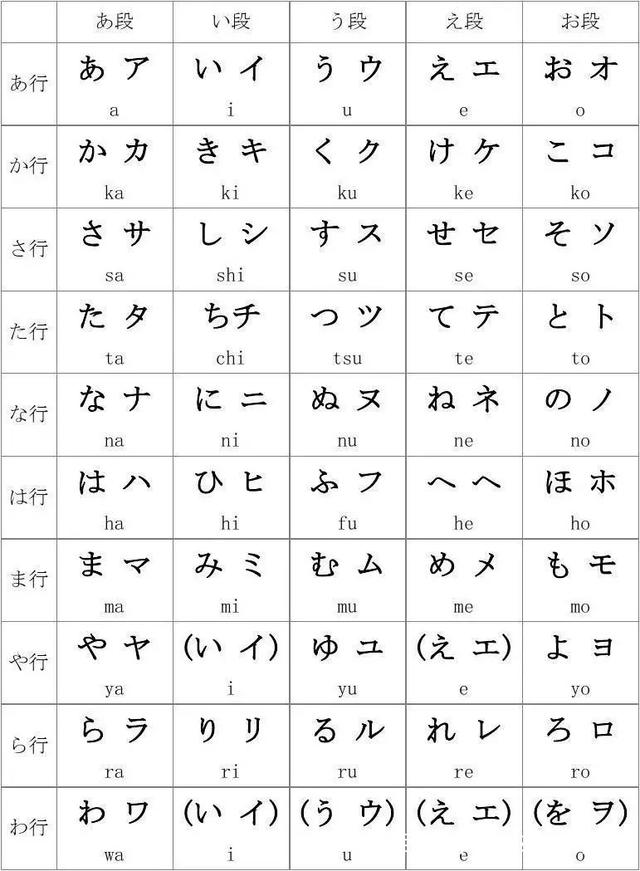
\includegraphics[width=0.85\linewidth]{五十音图.jpeg}
  \caption{五十音图。}
  \label{fig:phonetic}
\end{figure}

\begin{figure}[b]
  \centering
  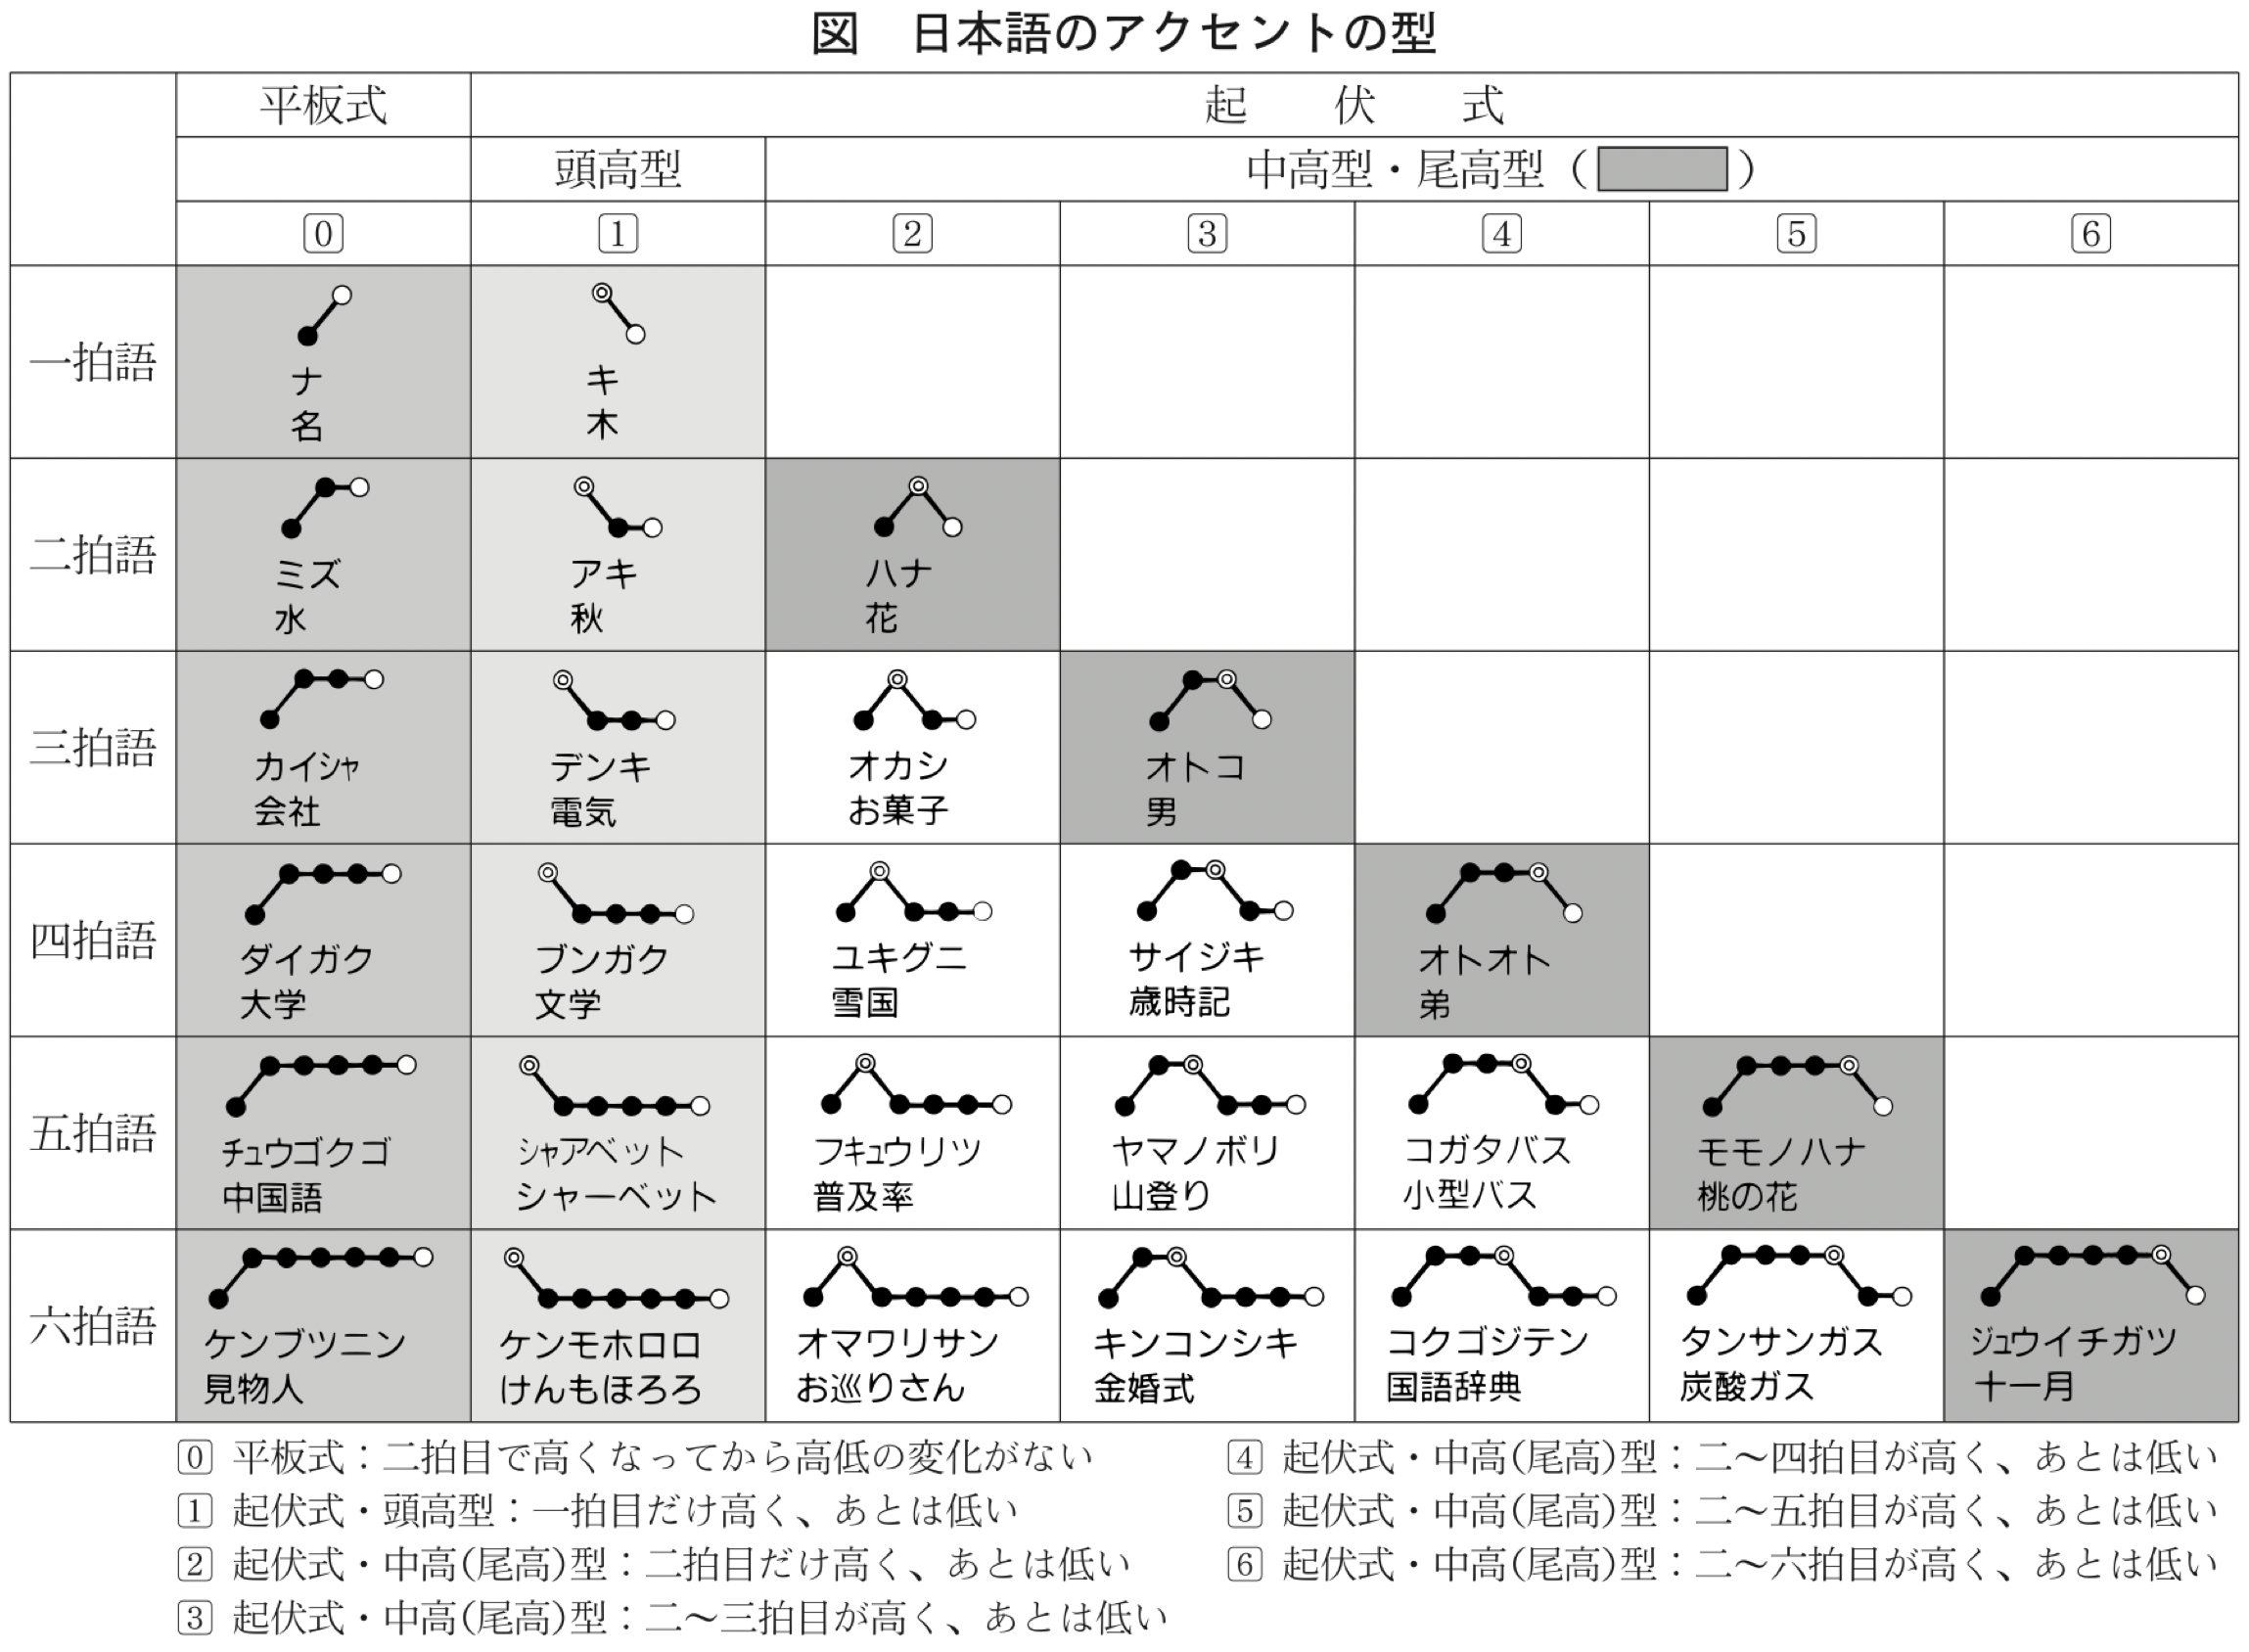
\includegraphics[width=0.90\linewidth]{accent.png}
  \caption{日语的音调。}
  \label{fig:phonetic}
\end{figure}


\clearpage

\section{常用词汇和表达}%
\label{sec:exp}

{\bf
\noindent 动词连用形+ています
}

接在持续性动词后,表示正在进行的动作或持续的状态。
\begin{itemize}
  \item 空港の到着ロビーで待っています。
\end{itemize}

{\bf
\noindent 动词连用形+てください
}

表示请求。
\begin{itemize}
  \item 書類にお名前を書いてください。
\end{itemize}

{\bf
\noindent 动词连用形+てから
}

表示一个动作完成后,再进行另一个动作。
\begin{itemize}
  \item 水泳をしてから、学校へ行きます。
\end{itemize}

{\bf
\noindent 体言+について
}

表示陈述的内容,相当于汉语``关于······''。
\begin{itemize}
  \item この問題について検討しましょう。
\end{itemize}

{\bf
\noindent 決して+用言否定式
}

表示强烈否定,相当于汉语``绝不······''。
\begin{itemize}
  \item 決して許しません。
\end{itemize}

{\bf
\noindent 体言+は言うまでもない
}

相当于汉语``不用说······''。
\begin{itemize}
  \item 英語は言うまでもなく、日本語もできます。
\end{itemize}

{\bf
\noindent 体言+という+体言
}

构成同位语。
\begin{itemize}
  \item 電車に乗ると、「携帯電話はご遠慮ください」という放送が聞こえます。
\end{itemize}


\begin{table}[h]
  \centering
  \caption{常用表达}
  \label{tab:label}
  \small
  \begin{tabular}{ll}
    初めましで & 初次见面 \\
    よろしく お願いします & 请多关照 \\
    今日は & 你好 \\
    すみません & 对不起 \\
    おはようございます & 早上好 \\
    お出掛けですか & 您出门啊 \\
    行って参ります & 我走了 \\
    おめでとうございます & 恭喜 \\
  \end{tabular}
\end{table}

\begin{table}[h]
  \centering
  \caption{常用指代词汇}
  \label{tab:label}
  \small
  \begin{tabular}{c|ccc|cc|c}
    & \multicolumn{3}{c|}{指示代词} & \multicolumn{2}{c|}{连体词} & 副词 \\
    & 事物 & 场所 & 方向 & 事物 & 性质状态 & 状态 \\
    \hline
    近 & これ & ここ   & こちら & この & こんな & こんなに \\
    中 & それ & そこ   & そちら & その & そんな & そんなに \\
    远 & あれ & あそこ & あちら & あの & あんな & あんなに \\
    ?  & どれ & どこ   & どちら & どの & どんな & どんなに \\
  \end{tabular}
\end{table}

\begin{table}[h]
  \centering
  \caption{人称代名詞}
  \label{tab:label}
  \small
  \begin{tabular}{c|c|c|ccc|c}
    & \multirow{2}{*}{第一人称} & \multirow{2}{*}{第二人称} & \multicolumn{3}{c|}{第三人称} & \multirow{2}{*}{不定称} \\
    & & & 近 & 中 & 远 & \\
    \hline
    单数 & わたし & あなた & このひと & そのひと & あのひと & どのひと \\
    复数 &わたしたち & あなたたち & このひとたち & そのひとたち & あのひとたち & どのひとたち \\
  \end{tabular}
\end{table}

\begin{table}[h]
  \centering
  \caption{常用数词}
  \label{tab:number}
  \small
  \begin{tabular}{ll | ll | ll}
    一 & いち \cn[2]                  & 百   &  ひゃく \cn[2]     & 一つ &  ひとつ \cn[2] \\
    二 & に \cn[1]                    & 三百 &  さんびゃく \cn[1] & 二つ &  ふたつ \cn[3] \\
    三 & さん \cn[0]                  & 六百 &  ろっぴゃく \cn[4] & 三つ &  みっつ \cn[3] \\
    四 & し \cn[1] $\,$ よん \cn[1]   & 八百 &  はっぴゃく \cn[4] & 四つ &  よっつ \cn[3] \\
    五 & ご \cn[1]                    & 千   &  せん \cn[1]       & 五つ &  いつつ \cn[2] \\
    六 & ろく \cn[2]                  & 三千 &  さんぜん \cn[3]   & 六つ &  むっつ \cn[3] \\
    七 & しち \cn[2] $\,$ なな \cn[1] & 八千 &  はっせん \cn[3]   & 七つ &  ななつ \cn[2] \\
    八 & はち \cn[2]                  & 万   &  まん \cn[1]       & 八つ &  やっつ \cn[3] \\
    九 & く \cn[1] $\,$ きゅう \cn[1] & 億   &  おく \cn[1]       & 九つ &  ここのつ \cn[2] \\
    十 & じゅう \cn[1]                &      &                    & 十つ &  とお \cn[1] \\
  \end{tabular}
\end{table}

\begin{table}[h]
  \centering
  \caption{常用量词}
  \label{tab:number}
  \small
  \begin{tabular}{lll | ll}
    人 & にん & 人           & 何人 & なんにん  \\
    時 & じ   & 点           & 何時 & なんじ    \\
    分 & ふん & 分           & 何分 & なんふん  \\
    番 & ばん & 第~         & 何番 & なんばん  \\
    枚 & まい & 张(扁平物) & 何枚 & なんまい  \\
    回 & かい & 回,次       & 何回 & なんかい  \\
    歳 & さい & 岁           & 何歳 & なんさい  \\
    冊 & さつ & 册           & 何冊 & なんさつ  \\
    本 & ほん & 根(细长物) & 何本 & なんほん  \\
    台 & だい & 台,辆       & 何台 & なんだい  \\
    足 & そく & 双           & 何足 & なんそく  \\
  \end{tabular}
\end{table}

\begin{table}[h]
  \centering
  \caption{日期}
  \label{tab:number}
  \small
  %\scriptsize
  \begin{tabular}{ll | ll | ll}
    一月   & いちがつ \cn[4]       & 一日     & ついたち \cn[4] & 日曜日 & にちようび \cn[3] \\
    二月   & にがつ \cn[3]         & 二日     & ふつか \cn[0]   & 月曜日 & げつうび   \cn[3] \\
    三月   & さんがつ \cn[1]       & 三日     & みっか \cn[0]   & 火曜日 & かようび   \cn[2] \\
    四月   & しがつ \cn[3]         & 四日     & よっか \cn[0]   & 水曜日 & すいようび \cn[3] \\
    五月   & ごがつ \cn[1]         & 五日     & いつか \cn[0]   & 木曜日 & もくようび \cn[3] \\
    六月   & ろくがつ \cn[0]       & 六日     & むいか \cn[0]   & 金曜日 & きんようび \cn[3] \\
    七月   & しちがつ \cn[0]       & 七日     & なのか \cn[0]   & 土曜日 & どようび   \cn[2] \\
    八月   & はちがつ \cn[4]       & 八日     & ようか \cn[0]   & 何曜日 & なんようび \cn[3] \\
    九月   & くがつ \cn[1]         & 九日     & ここのか \cn[0] &        & \\
    十月   & じゅうがつ \cn[4]     & 十日     & とおか \cn[0]   &        & \\
    十一月 & じゅういちがつ \cn[6] & 十四日   & じゅうよっか \cn[1] +\cn[0] &        & \\
    十二月 & じゅうにがつ \cn[5]   & 二十日   & はつか \cn[0]   &        & \\
    何月   & なんがつ \cn[1]       & 二十四日 & にじゅうよっか \cn[1] +\cn[0] &        & \\
    何年   & なんがつ \cn[1]       & 何日     & なんにち \cn[1] &        & \\
  \end{tabular}
\end{table}

\begin{table}[h]
  \centering
  \caption{地名}
  \label{tab:number}
  \small
  \begin{tabular}{lll | lll}
    名古屋 & なごや \cn[1]     & Nagoya  & 東京 & とうきょう \cn[0] & Tokyo \\
    仙台   & せんだい \cn[1]   & Sendai  & 沖縄 & おきなわ \cn[0]   & Okinawa \\
    新宿   & しんじゅく \cn[0] & Sinjuku & 原宿 & はらじゅく \cn[2] & Harajuku \\
  \end{tabular}
\end{table}

\begin{table}[h]
  \centering
  \caption{人名后缀}
  \label{tab:number}
  \small
  \begin{tabularx}{\textwidth}{llX}
    ちゃん & & 关系最为亲密的一种称呼,是「さん」的转音,接在名字后表示亲热。可以用在关系较好、彼此比较熟悉的朋友或夫妻、家人之间。 \\
    君 & くん & 称呼朋友或是年龄、资历比自己低的后辈时使用。常用于称呼男同学、男下属。
                带有亲密感,与「ちゃん」相比还略带一些敬意在里边,不熟悉的人之间一般不用。\\
    さん & & 相当于汉语中的 ``女士''、``先生''、``同志''、``同学'',日语语感中这个称呼既带有敬意也有亲密感在里边。\\
    様 & さま & 比「さん」更为敬重的一种表达,相当于汉语中的``大人''。多用于称呼比自己年长、地位较高的人。\\
    殿 & どの & 极为尊敬的一种用法,但是这种用法口语中不会使用,多用于奖状或毕业证等正式文书中。\\
    殿下 & でんか & 就是 ``殿下'' 的意思,是对皇太子、皇太子妃、皇太孙等皇室亲族的称呼。 \\
    陛下 & へいか & 对天皇以及皇后、太皇太后、皇太后的尊称。\\
  \end{tabularx}
\end{table}



\clearpage

\section{名詞}%

\subsection{形式名詞}%

形式上是名词,但却没有或很少有实质意义、
只能和修饰它的定语一起使用而不能独立使用的一类名词。

{\bf
\noindent つもり
}

表示计划或打算。
\begin{itemize}
  \item 私は日本へ行くつもりです。
\end{itemize}

{\bf
\noindent こと
}

泛指事情。
\begin{itemize}
  \item 冬は雪が降ることが多いです。
\end{itemize}

动词连体形+ことがあります,表示有时发生:
\begin{itemize}
  \item 私は東京へ出張に行くことがあります。
\end{itemize}

动词过去式+ことがあります,表示曾发生过:
\begin{itemize}
  \item 私は刺身お食べたことがあります。
\end{itemize}

{\bf
\noindent の
}

泛指人、事、物。
\begin{itemize}
  \item 留学が簡単なのはいいことです。
\end{itemize}

{\bf
\noindent ため
}

表示前项是后项的目标。
\begin{itemize}
  \item 人は食べるために生きるのではなく、生きるために食べるのです。
\end{itemize}

{\bf
\noindent はず
}

表示有把握的判断。
\begin{itemize}
  \item 電車は5時に来るはずだ。
  \item 彼にしらせたから、知っているはずだ。
\end{itemize}


\subsection{常见句型}%

{\bf
\noindent 体言+について
}

表示陈述的内容,相当于汉语``关于······''。
\begin{itemize}
  \item この問題について検討しましょう。
\end{itemize}


{\bf
\noindent 体言+は言うまでもない
}

相当于汉语``不用说······''。
\begin{itemize}
  \item 英語は言うまでもなく、日本語もできます。
\end{itemize}

{\bf
\noindent 体言+という+体言
}

构成同位语。
\begin{itemize}
  \item 電車に乗ると、「携帯電話はご遠慮ください」という放送が聞こえます。
\end{itemize}

{\bf
\noindent 体言+によって
}

相当于汉语``因······而异''。
\begin{itemize}
  \item 先生によって、教え方も違う。
\end{itemize}

{\bf
\noindent 体言+に対して
}

相当于汉语``对于······''。
\begin{itemize}
  \item その決定に対して抗議した。
\end{itemize}

{\bf
\noindent 体言+「とは」
}

提示主题,相当于汉语``所谓······''。
\begin{itemize}
  \item 週刊誌とは、毎週一回出る雑誌のことです。
\end{itemize}



\clearpage

\section{動詞}%


%%%%%%%%%%%%%%%%%%%%%%%%
\subsection{动词的分类}%
%%%%%%%%%%%%%%%%%%%%%%%%

\noindent 根据活用规律:五段动词、一段动词、サ变动词、カ变动词。

\noindent 根据是否要求宾语:他动词、自动词。

\noindent 根据后接「ている」的情况
\begin{itemize}
  \item 继续动词后接「ている」,表示动作正在进行:雁が大空を渡っている。
  \item 瞬间动词后接「ている」,表示动作已经结束但结果还保留着:小説発行の準備が始まっている。
  \item 形容词性动词后接「ている」,表示状态、性质。
\end{itemize}



%%%%%%%%%%%%%%%%%%%%%%%%%%
\subsection{动词的活用形}%
%%%%%%%%%%%%%%%%%%%%%%%%%%

动词的活用形见表~\ref{tab:verb}.

\begin{table}[htb]
  \centering
  \caption{动词活用示例}
  \label{tab:verb}
  \scriptsize
  \begin{tabular}{c | c | c | c c c c c c}
    分类 & 词例 & 词干 & 未然形 & 连用形 & 终止形 & 连体形 & 假定形 & 命令形 \\
    \hline
    \multirow{9}{*}{五段}
    & 書く & \ruby{書}{か}   & \makecell{\cn[1] か \\ \cn[2] こ} & き & く & く & け & け \\
    & 泳ぐ & \ruby{泳}{およ} & \makecell{\cn[1] が \\ \cn[2] ご} & ぎ & ぐ & ぐ & げ & げ \\
    & 話す & \ruby{話}{はな} & \makecell{\cn[1] さ \\ \cn[2] そ} & し & す & す & せ & せ \\
    & 立つ & \ruby{立}{た}   & \makecell{\cn[1] た \\ \cn[2] と} & ち & つ & つ & て & て \\
    & 取る & \ruby{取}{と}   & \makecell{\cn[1] ら \\ \cn[2] ろ} & り & る & る & れ & れ \\
    & 歌う & \ruby{歌}{うた} & \makecell{\cn[1] わ \\ \cn[2] お} & い & う & う & え & え \\
    & 死ぬ & \ruby{死}{し}   & \makecell{\cn[1] な \\ \cn[2] の} & に & ぬ & ぬ & ね & ね \\
    & 飛ぶ & \ruby{飛}{と}   & \makecell{\cn[1] ば \\ \cn[2] ぼ} & び & ぶ & ぶ & べ & べ \\
    & 読む & \ruby{読}{よ}   & \makecell{\cn[1] ま \\ \cn[2] も} & み & む & む & め & め \\
    \hline
    \multirow{2}{*}{上一段}
    & 起きる & \ruby{起}{お} & き & き & きる & きる & きれ & \makecell{きろ\\きよ} \\
    & 見る & \ruby{見}{み}   & み & み & みる & みる & みれ & \makecell{みろ\\みよ} \\
    \hline
    \multirow{2}{*}{下一段}
    & 食べる & \ruby{食}{た} & べ & べ & べる & べる & べれ & \makecell{べろ\\べよ} \\
    & 寝る & \ruby{寝}{ね}   & ね & ね & ねる & ねる & ねれ & \makecell{ねろ\\ねよ} \\
    \hline
    \multirow{2}{*}{サ变动词}
    & する &  & \makecell{し\\せ} & し & する & する & すれ & \makecell{しよ\\せよ} \\
    & 勉強する & \ruby{勉強}{べんきょう} & \makecell{し\\せ} & し & する & する & すれ & \makecell{しよ\\せよ} \\
    \hline
    カ变动词 & 来る & & \ruby{来}{こ} & \ruby{来}{き} & \ruby{来}{く}る & \ruby{来}{く}る & \ruby{来}{く}れ & \ruby{来}{こ}い \\
  \end{tabular}
\end{table}


\subsubsection{未然形}%
\label{ssub:_}

不能独立出现,必须后续助动词,才可表达完整的语法意义。
未然形后主要接一下几种助动词:
\begin{itemize}
  \item \cn[1] +「ない」,表示否定
  \item \cn[1] +「られる」等,构成不同的态
  \item \cn[2] +「う」、「よう」等,表示意志:私がご飯を作ろう。
\end{itemize}

{\bf
\noindent 決して+用言否定式
}

表示强烈否定,相当于汉语``绝不······''。
\begin{itemize}
  \item 決して許しません。
\end{itemize}

{\bf
\noindent 动词未然形+なければなりません
}

相当于汉语``必须······''。
\begin{itemize}
  \item 今週中に宿題を出さなければなりません。
  \item もう8時ですから、学校へ行かなければなりません。
\end{itemize}

{\bf
\noindent 动词未然形+ないでください
}

表示禁止,相当于汉语``请不要······''。
\begin{itemize}
  \item ここでタバコを吸わないでください。
  \item 授業の時間ですから、廊下で騒がないでください。
\end{itemize}


\subsubsection{连用形}%

\begin{enumerate}
  \item 充当名词或其他词素,构成复合词。
    \begin{itemize}
      \item 蒸し暑い
    \end{itemize}
  \item 表示中顿。
  \item 后接助动词「ます」、「た」、「たい」、「そうだ」等。
  \item 后接助词「に」、「て」、「たり」等。
\end{enumerate}

{\bf
\noindent 动词连用形+ています
}

接在持续性动词后,表示正在进行的动作或持续的状态。
\begin{itemize}
  \item 空港の到着ロビーで待っています。
\end{itemize}

{\bf
\noindent 动词连用形+てください
}

表示请求。
\begin{itemize}
  \item 書類にお名前を書いてください。
\end{itemize}

{\bf
\noindent 动词连用形+てから
}

表示一个动作完成后,再进行另一个动作。
\begin{itemize}
  \item 水泳をしてから、学校へ行きます。
\end{itemize}

{\bf
\noindent 动词、形容词连用形+てもいいです
}

表示许可,相当于汉语``可以······''。
\begin{itemize}
  \item この小説を借りてもいいですか。
  \item 明日は休みですから、遅くまで起きていてもいいです。
\end{itemize}

{\bf
\noindent 动词连用形+てはいけません
}

表示禁止,相当于汉语``不许······''。
\begin{itemize}
  \item 危ないから、そんなことをしてはいけません。
  \item 先生にそんなことを言ってはいけません。
\end{itemize}

{\bf
\noindent 动词连用形+てくる
}

表示时间或空间的发展或趋势,相当于汉语``······起来了''。
\begin{itemize}
  \item われわれの生活は日に日によくなってきた。
\end{itemize}

{\bf
\noindent 动词连用形+なさい
}

表示不客气的请求或命令,相当于汉语``你······吧''。
\begin{itemize}
  \item 早く帰りなさい。
\end{itemize}

{\bf
\noindent 动词连用形+「てはならない」
}

表示道理上不允许,相当于汉语``不可以······''。
\begin{itemize}
  \item 忙しくても、親に手紙を書くのを忘れてはならない。
\end{itemize}

{\bf
\noindent 动词连用形+「ていく」
}

表示动作、状态的发展趋势,相当于汉语``······起来''。
\begin{itemize}
  \item 少しずつ慣れていく。
\end{itemize}

{\bf
\noindent 动词连用形+「てしまう」
}

表示动作的完成。
\begin{itemize}
  \item 作文はもう書いてしまいました。
\end{itemize}

{\bf
\noindent 动词连用形+「ている」+「ところだ」
}

表示正在进行某一动作,相当于汉语``正在······''。
\begin{itemize}
  \item みんなは今、食事をしているところです。
\end{itemize}

{\bf
\noindent 动词连用形+「つつある」
}

表示动作持续进行,可用「ている」替换,用于书面。
\begin{itemize}
  \item 地球の環境はどんどん汚染されつつある。
\end{itemize}

{\bf
\noindent 动词连用形+「た」+「ところだ」
}

表示刚刚完成某一动作,相当于汉语``刚刚······''。
\begin{itemize}
  \item 飛行機は今、飛び立ったところです。
\end{itemize}

{\bf
\noindent 动词连用形+「てみる」
}

表示尝试做某事,相当于汉语``试着······''。
\begin{itemize}
  \item 自分で調べてみてください。
\end{itemize}

{\bf
\noindent 动词连用形+「てはいられない」
}

表示动作主体不能保持原来的状态,相当于汉语``不能······''。
\begin{itemize}
  \item もうこれ以上黙ってはいられない。
\end{itemize}

{\bf
\noindent 动词连用形+「た以上」
}

相当于汉语``既然······''。
\begin{itemize}
  \item 約束したた以上、守らなければならない。
\end{itemize}


\subsubsection{终止形}%

\begin{enumerate}
  \item 结句。
  \item 后接助动词。
  \item 后接助词。
\end{enumerate}

{\bf
\noindent 体言、用言终止形+かもしれません
}

表示对事物的估计,相当于汉语``也许······''。
\begin{itemize}
  \item 雨が降るかもしれません。
\end{itemize}

{\bf
\noindent 体言、用言终止形+に違いありません
}

表示确信,相当于汉语``一定是······''。
\begin{itemize}
  \item 彼はきっと成功するに違いありません。
\end{itemize}

{\bf
\noindent 用言终止形、体言+「とはいえ」
}

相当于汉语``虽然······,但是''。
\begin{itemize}
  \item 春とはいえ、まだ風が冷たい。
\end{itemize}

{\bf
\noindent 用言终止形、体言+「かどうか」
}

表示没有把握,相当于汉语``是否······''。
\begin{itemize}
  \item あの人が日本人かどうか私は知りません。
  \item 明日は雨が降るかどうかわかりません。
\end{itemize}


\subsubsection{连体形}%

\begin{enumerate}
  \item 后接体言,构成定语。
    \begin{itemize}
      \item 来る必要はありません。
    \end{itemize}
  \item 后接形式名词「こと」、「もの」等,将动词名词化。
    \begin{itemize}
      \item 早く起きることはいいことです。
    \end{itemize}
  \item 后接接续助词「ので」、「のに」等。
\end{enumerate}

{\bf
\noindent 体言の、用言连体形+ほうがいいです
}

多用于建议对方采取某种行为,相当于汉语``还是······为好''。
\begin{itemize}
  \item 明日は早く出発するから、早く寝たほうがいいです。
\end{itemize}

{\bf
\noindent 动词连体形+「に従って」
}

相当于汉语``随着······''。
\begin{itemize}
  \item 新しい技術の開発が進歩に従って、生産規模も拡大した。
\end{itemize}

{\bf
\noindent 动词连体形、体言+「につれて」
}

相当于汉语``随着······''。
\begin{itemize}
  \item 寮生活に慣れるにつれて、よく眠れるようになった。
\end{itemize}

{\bf
\noindent 动词连体形+「ところだ」
}

表示将要进行某一动作,相当于汉语``正要······''。
\begin{itemize}
  \item 今、出掛けるとこです。
\end{itemize}

{\bf
\noindent 动词连体形+「ことにする」
}

表示动作主体的主观决定,相当于汉语``决定······''。
\begin{itemize}
  \item 今度の夏休みに日本に旅行することにした。
\end{itemize}

{\bf
\noindent 动词连体形+「ことになる」
}

表示客观的决定、规定或自然产生的结果。
\begin{itemize}
  \item 彼は急に用事ができたので、私が一人で行くことになりました。
\end{itemize}


\subsubsection{假定形}%

后接接续助词「ば」,表示假定条件。
\begin{itemize}
  \item 明日雨が降れば、遠足をやめましょう。
\end{itemize}


\subsubsection{命令形}%

位于句末,表示命令。
\begin{itemize}
  \item もう一度読め。
  \item ただちに起きろ。
\end{itemize}



%%%%%%%%%%%%%%%%%%%%%%%%%%%%
\subsection{五段动词的音便}%
%%%%%%%%%%%%%%%%%%%%%%%%%%%%

五段动词的连用形在后接「て」、「ても」、「た」和「たり」时,
活用词尾要变成イ音便(カ行、ガ行)、促音便(タ行、ラ行、ワ行)和拨音便(ナ行、マ行、バ行)。

\begin{table}[h]
  \centering
  \caption{五段动词音便示例}
  \begin{tabular}{c | c | c | c c c c c c}
    分类 & 行 & 词例 & 词干 &  音便形 & 后续词 \\
    \hline
    \multirow{2}{*}{イ音便}
    & カ行 & 書く & \ruby{書}{か} & 書い & 書いて \\
    & ガ行 & 泳ぐ & \ruby{泳}{およ} & 泳い & 泳いで \\
    \hline
    \multirow{3}{*}{促音便}
    & タ行 & 立つ & \ruby{立}{た} & 立っ   & 立って \\
    & ラ行 & 取る & \ruby{取}{と} & 取っ   & 取って \\
    & ワ行 & 歌う & \ruby{歌}{うた} & 歌っ & 歌って \\
    \hline
    \multirow{3}{*}{拨音便}
    & ナ行 & 死ぬ & \ruby{死}{し} & 死ん & 死んで \\
    & マ行 & 読む & \ruby{読}{よ} & 読ん & 読んで \\
    & バ行 & 飛ぶ & \ruby{飛}{と} & 飛ん & 飛んで \\
  \end{tabular}
\end{table}



%%%%%%%%%%%%%%%%%%%%%%
\subsection{动词的态}%
%%%%%%%%%%%%%%%%%%%%%%

描述一件事情时,既可以从动作的施事者出发,
也可以从动作的受事者出发,
还可以从指使者出发。
由于动词所指动作与主语的关系所形成的谓语动词的形态变化,
叫做动词的``态''。
日语中动词的态有五类:主动态、被动态、使动态、可能态、自然发生态。

\subsubsection{被动态}%

当描述某一动作时,以承受者为主角进行描述,
该动词所表现的形态,就是被动态。

被动态的构成:
\begin{itemize}
  \item 五段动词未然形 \cn[1] + 「れる」
  \item 五段以外动词未然形+「られる」。
    其中サ变动词未然形+「られる」约音为「される」。
\end{itemize}

被动句中,谓语为动词被动态。
主语为动作的承受者或受害者,用「が」表示。
施事者以「--に」、「--から」等补语出现。

直接被动句,由他动词构成,可以还原为主动句:
\begin{itemize}
  \item 純子さんは先生に褒められた。
\end{itemize}

间接被动句,用自动词或他动词构成。
间接被动句中,
动词并没有直接作用于叙述的焦点,
而是句中的主语从动作施事者那里遭受到不利影响。
这里又分为两种情况,
一种是叙述的焦点与动作的施事者或承受者有必然联系:
\begin{itemize}
  \item 太郎はお母さんに日記を読まれた。
  \item 彼は二歳の時、両親に死なれな。
\end{itemize}
一种是两者没有必然联系,而是在叙述客观事实时偶然建立起了联系:
\begin{itemize}
  \item 私は帰る途中、雨に降られた。
\end{itemize}


\subsubsection{使动态}%

当描述某一动作时,以指使者、容许者为主角进行描述,
该动词所表现的形态,就是使动态。

使动态的构成:
\begin{itemize}
  \item 五段动词未然形 \cn[1] + 「せる」
  \item 五段以外动词未然形+「させる」。
    其中サ变动词未然形+「させる」约音为「される」。
\end{itemize}

使动句中,谓语为动词使动态。
主语是指使者,用「が」表示。
施事者以「--に」、「--を」等补语出现。

他动词的使动对象都用「--に」:
\begin{itemize}
  \item 先生が彼に論文を書かせる。
\end{itemize}

自动词的使动对象,表示强制性意思时用「--を」:
\begin{itemize}
  \item 子どもを9時までに寝させる。
\end{itemize}
表示非强制意思时用「--に」:
\begin{itemize}
  \item 小さい子どもに一人で大通りを渡らせるのは危ない。
\end{itemize}

被使动态,是使动态的被动态,描述的焦点是被指使者。


\subsubsection{可能态}%

当叙述焦点由动作本身转移到实现动作的能力或可能性时,
动作所发生的形态变化,称为可能态。

可能态的构成:
\begin{itemize}
  \item 一段动词+「られる」
  \item サ变动词词干+「できる」
  \item 动词连体形+「ことができる」
  \item 五段动词变为对应行的下一段动词
\end{itemize}

可能态的意义:
\begin{itemize}
  \item 表示能力:私は日本語お話すことがでけます。
  \item 表示可能性:用事があって出席できません。
  \item 表示许可:授業中は、大声で話すことができない。
\end{itemize}


\subsubsection{自然发生态}%

描述的焦点在于动作行为本身是自然而然的发生时,
动词的形态变化,就是自然发生态。

自然发生态的构成:
\begin{itemize}
  \item 五段动词未然形+「れる」
  \item 五段以外动词未然形+「れる」
\end{itemize}

自然发生态的意义:表示不由自主,
常用在人的感情、感觉、直觉、判断、思考的方面。
\begin{itemize}
  \item 日本料理は色が綺麗で、まるで芸術作品のように思われる。
  \item 雪が降ると、故郷のことが思い出される。
\end{itemize}



%%%%%%%%%%%%%%%%%%%%%%
\subsection{授受動詞}%
%%%%%%%%%%%%%%%%%%%%%%

授受动词共有7个,分为3组:
\begin{itemize}
  \item 他方授我方:「くれる」(尊敬语「くださる」)
  \item 我方授他方:「やる」、「あげる」(谦让语「差し上げる」)
  \item 我方受他方:「もらう」(谦让语「いただく」)
\end{itemize}

例句:
\begin{itemize}
  \item 友達が(私に)辞書をくれた。
  \item (私は)友達に辞書をもらった。
  \item 社長が弟にネクタイをくださった。
  \item 弟が社長にネクタイをいただいた。
  \item 兄が弟に500$やった。
  \item 兄が友達に時計おあげた。
  \item 兄が社長にお酒お差し上げた。
\end{itemize}


\subsubsection{作为补助动词的授受动词}%

动词连用形+「て」+授受动词,表示人物之间行为的往来与恩惠关系。
\begin{itemize}
  \item 駅まで送ってくれました。
  \item いろいろと手伝ってくれました。
  \item 弟の勉強を手伝ってやりました。
  \item 何もしてあげませんでした。
  \item この本を貸してあげましょう。
  \item 中村さんに絵を書いてもらいました。
\end{itemize}




\clearpage

\section{形容詞}%

\subsection{形容词的分类}%

\noindent 属性形容詞:表示事物的客观属性、状态。

\noindent 感情形容詞:表示人的喜怒哀乐、爱憎好恶等感情、心理感受,或是疼痛、冷热等身体感觉。


\subsection{形容词的活用}%

\begin{table}[h]
  \centering
  \caption{形容词活用示例}
  \begin{tabular}{c | c | c c c c c}
    词例 & 词干 & 未然形 & 连用形 & 终止形 & 连体形 & 假定形 \\
    \hline
    暑い & 暑 & かろ & \makecell{\cn[1] く \\ \cn[2] かっ} & い & い & けれ \\
  \end{tabular}
\end{table}

{\bf
\noindent 未然形
}

后接推测助动词「う」,构成简体推量形式,表示推测。
\begin{itemize}
  \item 明日も 暑かろう。
\end{itemize}

{\bf
\noindent 连用形「く」
}

置于所修饰用言前作状语。
\begin{itemize}
  \item 速く 食べます。
\end{itemize}

与「なる」或「する」结合表示变化。
此时,「形容词连用形+なる」可以看作一个自动词,表示客观变化。
「形容词连用形+する」可以看作一个他动词,表示人为地改变。
\begin{itemize}
  \item 人口が增え、市場も大きくなった。
\end{itemize}

两个用言连用时表示中顿。
\begin{itemize}
  \item この部屋は 広くて明るい。
\end{itemize}

后接补助形容词「ない」表示否定。
\begin{itemize}
  \item 今日の天気は よくない。
\end{itemize}

{\bf
\noindent 连用形「かっ」
}

后接过去完了助动词「た」。
\begin{itemize}
  \item 昨日の天気は よかった。
\end{itemize}

{\bf
\noindent 终止形
}

作谓语结句。

后接助词「から」、「けれども」、「し」、「か」、「よ」、「ね」等。

{\bf
\noindent 连体形
}

后接体言作定语。
\begin{itemize}
  \item 面白い映画を みます。
\end{itemize}

{\bf
\noindent 假定形
}

后接接续助词「ば」,表示假定条件。
\begin{itemize}
  \item 美味しければ 食べます。
\end{itemize}


\subsection{補助形容詞}%

接在其它用言后起补助作用的形容词,包括「ない」、「ほしい」、「いい」。

{\bf
\noindent ない
}

接在形容词、形容动词、形容词型助词、形容词型助动词的连用形之后,
表示否定。

{\bf
\noindent ほしい
}

接在「用言连用形+て」或「用言未然形+ないで」后,
表示说话人希望出现某一事态。

{\bf
\noindent いい
}



\clearpage

\section{形容動詞}%

\subsection{形容动词的分类}%

\noindent 属性形容動詞。

\noindent 感情形容動詞。


\subsection{形容动词的活用}%

\begin{table}[h]
  \centering
  \caption{形容动词活用示例}
  \begin{tabular}{c | c | c c c c c}
    词例 & 词干 & 未然形 & 连用形 & 终止形 & 连体形 & 假定形 \\
    \hline
    静かだ & 静か & だろ & \makecell{\cn[1] で \\ \cn[2] に \\ \cn[3] だっ} & だ & な & なら \\
  \end{tabular}
\end{table}

{\bf
\noindent 未然形
}

后接推测助动词「う」,表示推测。
\begin{itemize}
  \item 駅前は 夜も にぎやかだろう。
\end{itemize}

{\bf
\noindent 连用形「で」
}

置于所修饰用言前作状语。
\begin{itemize}
  \item 速く 食べます。
\end{itemize}

与「なる」或「する」结合表示变化。
此时,「形容词连用形+なる」可以看作一个自动词,表示客观变化。
「形容词连用形+する」可以看作一个他动词,表示人为地改变。
\begin{itemize}
  \item 人口が增え、市場も大きくなった。
\end{itemize}

两个用言连用时表示中顿。
\begin{itemize}
  \item この部屋は 静かで きれいです。
\end{itemize}

后接补助形容词「ない」表示否定。
\begin{itemize}
  \item あまり好きではないが、さほど嫌いでもない。
\end{itemize}

{\bf
\noindent 连用形「に」
}

修饰后续用言,作状语。
\begin{itemize}
  \item 部屋を きれいに 掃除しました。
\end{itemize}

与「なる」或「する」结合表示变化。
此时,「形容词连用形+なる」可以看作一个自动词,表示客观变化。
「形容词连用形+する」可以看作一个他动词,表示人为地改变。
\begin{itemize}
  \item 人口が增え、市場も大きくなった。
\end{itemize}

{\bf
\noindent 连用形「だっ」
}

后接过去完了助动词「た」。
\begin{itemize}
  \item 昨日は 暇だった。
\end{itemize}

{\bf
\noindent 终止形
}

作谓语结句。

后接助词「から」、「けれども」、「し」等。

{\bf
\noindent 连体形
}

后接体言作定语。
\begin{itemize}
  \item 図書館は 静かな所です。
\end{itemize}

{\bf
\noindent 假定形
}

后接接续助词「ば」,表示假定条件。
\begin{itemize}
  \item そこが 静かなら そこで 勉強します。
\end{itemize}


\clearpage

\section{助動詞}%

有形态变化的功能词。
主要接在以动词为主的用言后,
从时、态等方面对用言加以补充,
或增添各种表示陈述方式等的意义。

\subsection{表示态的助动词}%

\subsubsection{れる、られる}%

接在动词未然形后构成动词的被动态,属于下一段动词型活用。

\begin{table}[h]
  \centering
  \caption{「れる」、「られる」活用示例}
  \begin{tabular}{c c c c c c c}
    基本形 & 未然形 & 连用形 & 终止形 & 连体形 & 假定形 & 命令形 \\
    \hline
    れる & れ & れ & れる & れる & れれ & \makecell{れろ \\ れよ} \\
    られる & られ & られ & られる & られる & られれ & \makecell{られろ \\ られよ} \\
  \end{tabular}
\end{table}

\subsection{表示时的助动词}

过去完了助动词「た」,
主要用来构成过去时,
表示完成。
接在用言、助动词的连用形后。
「た」属于特殊活用。

\begin{table}[h]
  \centering
  \caption{「た」活用示例}
  \begin{tabular}{c c c c c c c}
    基本形 & 未然形 & 连用形 & 终止形 & 连体形 & 假定形 & 命令形 \\
    \hline
    た & たろ & & た & た & たら & \\
  \end{tabular}
\end{table}


\subsection{构成敬体的助动词}%

\subsubsection{ます}%

接在动词和动词型助动词的连用形之后,
表示说话者和作者的一种郑重的心情,
表示对听者和读者的尊敬,
构成敬体。
广泛用于谈话中。

「ます」属于特殊活用。

\begin{table}[h]
  \centering
  \caption{「ます」活用示例}
  \begin{tabular}{c c c c c c c}
    基本形 & 未然形 & 连用形 & 终止形 & 连体形 & 假定形 & 命令形 \\
    \hline
    ます & \makecell{ませ \\ ましょ} & まし & ます & ます & ますれ & \makecell{ませ \\ まし} \\
  \end{tabular}
\end{table}

\begin{itemize}
  \item 私わ お茶を飲みません。
  \item みんなもう帰りました。
  \item 毎日、六時に起きます。
  \item いらっしゃいませ。
\end{itemize}


\subsubsection{です}%

接在形容词、形容词型助动词之后,
表示说话者和作者的一种郑重的心情,
表示对听者和读者的尊敬,
构成敬体。

「ます」属于特殊活用,一般只使用其未然形和终止形。

\begin{table}[h]
  \centering
  \caption{「です」活用示例}
  \begin{tabular}{c c c c c c c}
    基本形 & 未然形 & 终止形 \\
    \hline
    です & でしょ & です \\
  \end{tabular}
\end{table}



\subsection{表示各种陈述方式的助动词}%

\subsubsection{たい、たがる}%

接在动词的连用形之后,
表示说话人内心的愿望,
相当于汉语``想······''。
「たい」表示说话人内心的愿望,通常用于第一人称。
「たがる」表示显露与言行的愿望,通常用于第三人称。

「たい」属于形容词型活用,
「たがる」属于五段动词型活用。

\begin{table}[h]
  \centering
  \caption{「たい」活用示例}
  \begin{tabular}{c | c | c c c c c}
    基本形 & 未然形 & 连用形 & 终止形 & 连体形 & 假定形 \\
    \hline
    たい & たかろ & \makecell{\cn[1] たく \\ \cn[2] たかっ} & たい & たい & たけれ \\
    たがる & \makecell{\cn[1] たがら \\ \cn[2] たがろ} & \makecell{\cn[1] たがり \\ \cn[2] たがっ} & たがる & たがる & たがれ \\
  \end{tabular}
\end{table}

\begin{itemize}
  \item 早く帰りたかろう。
  \item 私は 薬を飲みたくないです。
  \item 昨日、家へ帰りたかったです。
  \item 子供はお菓子を食べだかっています。
\end{itemize}


\subsubsection{ない}%

接在动词的未然形之后,
表示对动作、作用、状态、属性的否定,
相当于汉语``不······''。

「ない」属于形容词型活用。

\begin{table}[h]
  \centering
  \caption{「たい」活用示例}
  \begin{tabular}{c | c | c c c c c}
    基本形 & 未然形 & 连用形 & 终止形 & 连体形 & 假定形 \\
    \hline
    ない & なかろ & \makecell{\cn[1] なく \\ \cn[2] なかっ} & ない & ない & なけれ \\
  \end{tabular}
\end{table}

\begin{itemize}
  \item 私はそのことを何も知らない。
\end{itemize}

\subsubsection{である}

断定助动词,接在体言后,表示对事物的断定,属于文章语。
词尾变化同五段动词。
否定式为「ではない」。
\begin{itemize}
  \item 鯨は哺乳動物であり、魚類ではない。
\end{itemize}





\clearpage

\section{助詞}%


%%%%%%%%%%%%%%%%%%%%
\subsection{格助詞}%
%%%%%%%%%%%%%%%%%%%%

\subsubsection{が}%

\begin{enumerate}
  \item 表示主语:銀行が あります。
\end{enumerate}


\subsubsection{を}%

\begin{enumerate}
  \item 表示宾语:私は よくインターネットをします。
\end{enumerate}


\subsubsection{の}%

\begin{enumerate}
  \item 表示定语:私はの名前は 陳紅です。
  \item 表示定语从句中的主语:英語の話せる人はいますか。
\end{enumerate}


\subsubsection{に}%

\begin{enumerate}
  \item 表示存在的场所:冷蔵庫に あります。
  \item 表示动作的时间:八時に 授業が あります。
  \item 表示比较的基准:運動は 体に いいです。\\ 
    弟は 一日に二時間 本を読みます。\\
    日本の若者にとって、留学は珍しいことではありません。
  \item 表示动作涉及的对象:両親に 電話します。
\end{enumerate}


\subsubsection{より}%

\begin{enumerate}
  \item 表示比较的基准:銀行は 郵便局より 近いです。
\end{enumerate}


\subsubsection{で}%

\begin{enumerate}
  \item 表示动作发生的场所:教室で 宿題をします。
  \item 表示进行动作的手段:万年筆で 手紙を書きます。
  \item 表示范围:日本では 富士山が いちぼん 高いです。
\end{enumerate}


\subsubsection{と}%

\begin{enumerate}
  \item 表示动作的共同者:友達と 昼ご飯を食べます。
  \item 表示思考、叙述的内容:私は彼が来ると思います。\\
    田中さんはお金を持っていると言いました。
\end{enumerate}


\subsubsection{から}%

\begin{enumerate}
  \item 表示动作的起点:朝から彼を待ている。
  \item 表示原因:用事があるから、明日の会議には出席できません。
\end{enumerate}


\subsubsection{まで}%

\begin{enumerate}
  \item 表示动作的终点:デパートは 何時までですか。
\end{enumerate}


\subsubsection{へ}%

\begin{enumerate}
  \item 表示动作的方向:今日 王さんは学校へ勉強に来ました。
  \item 表示动作的对象:これは母への手紙です。
\end{enumerate}



%%%%%%%%%%%%%%%%%%%%%%
\subsection{語気助詞}%
%%%%%%%%%%%%%%%%%%%%%%

\subsubsection{か}%

\begin{enumerate}
  \item 表示疑问:それは なんですか?
\end{enumerate}


\subsubsection{ね}%

\begin{enumerate}
  \item 表示感叹:王さんは 日本語が お上手ですね。
\end{enumerate}


\subsubsection{よ}%

\begin{enumerate}
  \item 表示判断,主张或提醒对方注意:明日、李さんも 行きますよ。
\end{enumerate}


\subsubsection{な}%

接在动词终止形之后,表示禁止:
\begin{enumerate}
  \item そんな冗談を言うな。
\end{enumerate}


\subsubsection{かな}%

接在体言、用言终止形后,
表示疑问或愿望。
\begin{itemize}
  \item これでいいかな。
  \item 早く夏休みにならないかな。
\end{itemize}


%%%%%%%%%%%%%%%%%%%%%%
\subsection{並立助詞}%
%%%%%%%%%%%%%%%%%%%%%%

并列助词用来并列两个或两个以上的处于同等地位的内容词或词组,
构成联合式词组。
所构成的联合式词组,
不具备``格'',不能体现这个联合式词组在句中的地位及其与其他词的关系,
必须借助加在其后的格助词构成主宾补定语等成分,
或加助动词构成谓语成分。


\subsubsection{と}%

\begin{enumerate}
  \item 表示并列,列举事物的全部:私は 兄と姉が います。
\end{enumerate}


\subsubsection{や}%

\begin{enumerate}
  \item 表示列举,列举全体的一部分:郵便局には 雑誌や新聞が あります。
\end{enumerate}


\subsubsection{たり}%

接在用言连用形后,
表示动作在某一时间内交替进行或状态交替出现。
构成的联合式词组具有体言的性质,
还可以后接「する」像サ变动词词干使用,
或者直接如句作状语。

\begin{enumerate}
  \item 寒かったり暑かったり
\end{enumerate}


\subsubsection{とか}%

接在体言、用言终止形后,
表示列举性的并列。
\begin{itemize}
  \item 暇の時は散歩するとか、スポーツをするとかします。
\end{itemize}


%%%%%%%%%%%%%%%%%%%%%%
\subsection{提示助詞}%
%%%%%%%%%%%%%%%%%%%%%%

\subsubsection{も}%

\begin{enumerate}
  \item 表示同类事物的追加:私も 一人っ子です。
  \item 表示强调:昨日の晩餐会には、お貴客さんが50人も来ました。
\end{enumerate}


\subsubsection{しか}%

接在体言后。
\begin{enumerate}
  \item 表示限定某一事物,对除此以外的一切事物都加以否定,与否定形式的谓语呼应:
    彼は小説しか読まない。\\
    教室には一人しかいない。
\end{enumerate}


%%%%%%%%%%%%%%%%%%%%%%
\subsection{副助詞}%
%%%%%%%%%%%%%%%%%%%%%%

副助词接在体言、相当于体言的词语后。
与其所附属的内容词作状语,修饰后面的用言。


\subsubsection{ほど}%

\begin{enumerate}
  \item 表示比较的基准:今日は 昨日ほど 忙しく ありません。
\end{enumerate}


\subsubsection{くらい}%

\begin{enumerate}
  \item 表示概数:月に 三回くらい 電話をします。
\end{enumerate}


\subsubsection{か}%

接在体言后。
\begin{enumerate}
  \item 表示不确定的事物:何人かで行く。
\end{enumerate}


\subsubsection{だけ}%

接在体言、用言连体形后。
\begin{enumerate}
  \item 表示限定:あなただけが知っているでしょう。\\
    こプールは夏の間だけ開きます。
\end{enumerate}


\subsubsection{ごとに}%

接在体言后。
\begin{itemize}
  \item 相当于汉语``每······'': 三時間ごとに注射する。
\end{itemize}


\subsubsection{ずつ}%

接在表示数量、程度的体言和副词、助词后,
表示按同样的数量分配或同样的程度反复。
\begin{itemize}
  \item 毎朝一本ずつ牛乳を飲む。
  \item 新しい地下鉄や道路も少しずつ造っています。
\end{itemize}


\subsubsection{まで}%

接在体言、用言连体形后,
表示程度,或提出一个极端事例以暗示其他:
\begin{itemize}
  \item そんなことまで心配しないでください。
  \item お母さんまで私たちの結婚に反対している。
\end{itemize}


%%%%%%%%%%%%%%%%%%%%%%
\subsection{接続助詞}%
%%%%%%%%%%%%%%%%%%%%%%

接续助词连接用言、用言性词组,
表示它们之间的关系,
在句子中起承上启下的作用。


\subsubsection{が}%

\begin{enumerate}
  \item 表示转折:勉強は 忙しいですが、楽しいです。
\end{enumerate}


\subsubsection{ので}%

接在用言、助动词的连体形后。
\begin{enumerate}
  \item 表示客观的因果关系:彼は若いので、元気があります。
\end{enumerate}


\subsubsection{て}%

接在动词、形容词、助动词的连用形之后。
\begin{enumerate}
  \item 表示并列:この川は長くて広いです。
  \item 表示动作的先后关系:夏は過ぎて秋が来た。
  \item 表示动作进行的方式:父は毎日電車に乗って会社へ行きます。
  \item 表示原因:熱があって、学校を休みました。
\end{enumerate}


\subsubsection{ても(でも)}%

「ても」接在动词、形容词、助动词的连用形之后,
「でも」接在名词、形容动词词干后,
表示让步条件的逆态接续,
相当于汉语``即使······也······''。
\begin{itemize}
  \item たとえ雨が降っても、行きます。
  \item 雪は夜になってもやみませんでした。
  \item それは子供でもできる問題です。
  \item スーパーマーケットでは何でも売っています。
\end{itemize}


\subsubsection{けれども}%

接在用言、助动词的终止形后。
\begin{itemize}
  \item 表示转折:話せるけれども、書けない。
\end{itemize}


\subsubsection{ながら}%

接在动词连用形后。
\begin{itemize}
  \item 表示动作同时进行:あの人はいつも新聞を読みながら、ご飯を食べます。
\end{itemize}


\subsubsection{し}%

接在用言终止形后。
\begin{itemize}
  \item 表示两个事项同时存在:この花は色も綺麗だし、香りもいいです。
\end{itemize}


\subsubsection{のに}%

接在用言、助动词的连体形或终止形之后,
连接两个事项,
表示转折,有时带有出乎意料、埋怨、责怪等语感。
\begin{itemize}
  \item 今日は日曜日なのに、人出が少ない。
  \item 雨が降っているのに、外で遊んでいる。
\end{itemize}

\clearpage

\section{文}%
\label{sec:_}

%%%%%%%%%%%%%%%%%%%%
\subsection{断定文}%
%%%%%%%%%%%%%%%%%%%%

{\bf
\noindent 体言は 体言です

\noindent 体言は 体言ではありません
}

\begin{enumerate}
  \item 私わ 大学院生です。
  \item 彼女わ 主婦では ありません。
  \item 田中さんは 先生でしょう。
  \item 今日は 水曜日で、昨日は 火曜日でした。
  \item 昨日は 休みでは ありませんでした。
\end{enumerate}


%%%%%%%%%%%%%%%%%%%%
\subsection{描写文}%
%%%%%%%%%%%%%%%%%%%%

{\bf
\noindent 体言は 形容詞です
}

\begin{enumerate}
  \item 東京の夏は 蒸し暑いです。
\end{enumerate}

{\bf
\noindent 体言は 形容動詞
\noindent 体言は 形容動詞词干です
}

\begin{enumerate}
  \item 街は 清潔です。
\end{enumerate}


%%%%%%%%%%%%%%%%%%%%
\subsection{叙述文}%
%%%%%%%%%%%%%%%%%%%%

{\bf
\noindent 体言は 動詞
}

\begin{enumerate}
  \item 私は 六時に 起きます。
  \item 教室で 予習を します。
\end{enumerate}


%%%%%%%%%%%%%%%%%%%%
\subsection{存在文}%
%%%%%%%%%%%%%%%%%%%%

{\bf
\noindent 体言は 体言にあります

\noindent 体言は 体言にいます
}

\begin{enumerate}
  \item 兄は 名古屋に います。
  \item 花瓶は 机の上に あります。
  \item 実験室は どこに ありますか。
\end{enumerate}

{\bf
\noindent 体言には 体言があります

\noindent 体言には 体言がいます
}

\begin{enumerate}
  \item 学校には 図書館が あります。
  \item 部屋の中には 猫が いますか?
\end{enumerate}


\clearpage

\twocolumn
\setlength{\columnseprule}{0.4pt}
\section{新しい単語}%
\label{sec:words}

%%%%%%%%%%%%%%%%%%
\subsection{名詞}%
%%%%%%%%%%%%%%%%%%

\footnotesize
\begin{supertabular}{lll}
  本文     & ほんぶん \cn[1] & 正文 \\
  学生     & がくせい \cn[0] & 学生 \\
  学部     & がくぶ \cn[0] & 系 \\
  大学     & だいがく \cn[0] & 大学 \\
  大学院   & だいがくいん \cn[4] & 研究生院 \\
  大学院生 & だいがくいんせい \cn[4] & 研究生 \\
  大学生   & だいがくせい \cn[4] & 大学生 \\
  高校生   & こうこうせい \cn[3] & 高中生 \\
  中学生   & ちゅうがくせい \cn[4] & 初中生 \\
  小学生   & しょうがくせい \cn[4] & 小学生 \\
  同級生   & どうきゅうせい \cn[3] & 同年级生 \\
  授業     & じゅぎょう \cn[1] & 上课 \\
  放課後   & ほうかご \cn[0] & 放学后 \\
  宿題     & しゅくだい \cn[0] & 作业 \\
  予習     & よしゅう \cn[0] & 预习 \\
  寮       & りょう \cn[1] & 宿舍 \\
  消灯     & しょうとう \cn[0] & 熄灯 \\
  夏休み   & なつやすみ \cn[3] & 暑假 \\
  試験     & しけん \cn[2] & 考试 \\
  出身     & しゅっしん \cn[0] & 出生地 \\
  皆       & みな \cn[2] & 大家 \\
  主婦     & しゅふ \cn[1] & 家庭主妇 \\
  看護婦   & かんごふ \cn[3] & 护士 \\
  会社員   & かいしゃいん \cn[3] & 公司职员 \\
  以前     & いぜん \cn[1] & 以前 \\
  現在     & げんざい \cn[1] & 现在 \\
  名前     & なまえ \cn[0] & 名字 \\
  専攻     & せんこう \cn[0] & 专业 \\
  中国語   & ちゅごくご \cn[0] & 中文 \\
  外国語   & がいこくご \cn[0] & 外语 \\
  中国人   & ちゅごくじん \cn[4] & 中国人 \\
  日本人   & にほんじん \cn[4] & 日本人 \\
  趣味     & しゅみ \cn[1] & 爱好 \\
  実験室   & じっけんしつ \cn[3] & 实验室 \\
  隣       & となり \cn[0] & 旁边 \\
  近く     & ちかく \cn[2] & 附近 \\
  中       & なか \cn[1] & 中 \\
  先生     & せんせい \cn[3] & 老师 \\
  友達     & ともだち \cn[0] & 朋友 \\
  親友     & しんゆう \cn[0] & 好友 \\
  両親     & りょうしん \cn[1] & 父母 \\
  父       & ちち \cn[2] & 父亲 \\
  母       & はは \cn[1] & 母亲 \\
  兄       & あに \cn[1] & 哥哥 \\
  弟       & おとうと \cn[4] & 弟弟 \\
  姉       & あね \cn[0] & 姐姐 \\
  妹       & いもうと \cn[4] & 妹妹 \\
  祖父母   & そふぼ \cn[2] & 祖父母 \\
  兄弟     & きょうだい \cn[1] & 兄弟姐妹 \\
  実家     & じっか \cn[0] & 父母家 \\
  来年     & らいねん \cn[0] & 明年 \\
  定年     & ていねん \cn[0] & 退休年龄 \\
  帰宅     & きたく \cn[0] & 回家 \\
  午前     & ごぜん \cn[1] & 上午 \\
  正午     & しょうご \cn[1] & 中午 \\
  午後     & ごご \cn[1] & 下午 \\
  夜       & よる \cn[1] & 夜晚 \\
  日       & ひ \cn[0] & 日子 \\
  将来     & しょうらい \cn[1] & 将来 \\
  時代     & じだい \cn[0] & 时代 \\
  週       & しゅう \cn[1] & 周 \\
  週末     & しゅうまつ \cn[0] & 周末 \\
  毎日     & まいにち \cn[1] & 每天 \\
  日々     & ひび \cn[1] & 每天 \\
  一日     & いちにち \cn[4] & 一天 \\
  毎朝     & まいあさ \cn[1] & 每天早晨 \\
  朝ご飯   & あさごはん \cn[3] & 早饭 \\
  昼ご飯   & ひるごはん \cn[3] & 午饭 \\
  晩ご飯   & ばんごはん \cn[3] & 晚饭 \\
  住居     & じゅうきょ \cn[1] & 住所 \\
  郵便局   & ゆうびんきょく \cn[3] & 邮局 \\
  銀行     & ぎんこう \cn[0] & 银行 \\
  映画館   & えいがかん \cn[3] & 电影院 \\
  食堂     & しょくどう \cn[0] & 食堂 \\
  喫茶店   & きっさてん \cn[0] & 咖啡馆 \\
  公園     & こうえん \cn[0] & 公园 \\
  空港     & くうこう \cn[0] & 机场 \\
  お手洗い & おてあらい \cn[3] & 洗手间 \\
  砂糖     & さとう \cn[2] & 砂糖 \\
  四季     & しき \cn[2] & 四季 \\
  季節     & きせつ \cn[2] & 季节 \\
  春       & はる \cn[1] & 春 \\
  夏       & なつ \cn[2] & 夏 \\
  秋       & あき \cn[1] & 秋 \\
  冬       & ふゆ \cn[2] & 冬 \\
  雨       & あめ \cn[1] & 雨 \\
  雪       & ゆき \cn[2] & 雪 \\
  風       & ふう \cn[1] & 风 \\
  魅力     & みりょく \cn[0] & 魅力 \\
  花見     & はなみ \cn[3] & 赏花 \\
  桜       & さくら \cn[0] & 樱花 \\
  紅葉     & こうよう \cn[0] & 红叶 \\
  富士山   & ふじさん \cn[1] & 富士山 \\
  初め     & はじめ \cn[0] & 最初 \\
  海       & うみ \cn[1] & 海 \\
  海岸     & かいがん \cn[0] & 海岸 \\
  人気     & にんき \cn[0] & 人气 \\
  仕事     & しごと \cn[0] & 工作 \\
  仕方     & しかた \cn[0] & 方法 \\
  首都     & しゅと \cn[1] & 首都 \\
  人口     & じんこう \cn[0] & 人口 \\
  都市     & とし \cn[1] & 都市 \\
  交通     & こうつう \cn[0] & 交通 \\
  町       & まち \cn[2] & 城镇 \\
  高層     & こうそう \cn[0] & 高楼 \\
  若者     & わかもの \cn[0] & 年轻人 \\
  問題     & もんだい \cn[0] & 问题 \\
  地震     & じしん \cn[0] & 地震 \\
  物価     & ぶっか \cn[0] & 价格 \\
  人々     & ひとびと \cn[2] & 人们 \\
  水泳     & すいえい \cn[0] & 游泳 \\
  顔      & かお \cn[0] & 脸 \\
  喉       & のど \cn[1] & 嗓子 \\
  音楽     & おんがく \cn[1] & 音乐 \\
  洗濯     & せんたく \cn[0] & 洗衣服 \\
  家庭     & かてい \cn[0] & 家庭 \\
  教師     & きょうし \cn[1] & 教师 \\
  アルバイト & \cn[3] & 兼职 \\
  あと     & \cn[1] & 后 \\
  久しぶり & ひさしぶり \cn[0] & 许久 \\
  写真     & しゃしん \cn[0] & 照片 \\
  代わり   & かわり \cn[0] & 代替 \\
  お互い   & おたがい \cn[0] & 互相 \\
  迎え     & むかえ \cn[0] & 迎接 \\
  海外     & かいがい \cn[1] & 海外 \\
  国内     & こくない \cn[2] & 国内 \\
  各地     & かくち \cn[1] & 各地 \\
  事       & こと \cn[2] & 事情 \\
  新婚     & しんこん \cn[0] & 新婚 \\
  短期     & たんき \cn[1] & 短期 \\
  個人     & こじん \cn[1] & 个人 \\
  大勢     & おおぜい \cn[3] & 多数 \\
  国       & くに \cn[0] & 国家 \\
  方       & ほう \cn[1] & 方面 \\
  値段     & ねいだん \cn[0] & 价格 \\
  場合     & ばあい \cn[0] & 场合 \\
  青春     & せいしゅん \cn[0] & 青春 \\
  お盆     & おぼん \cn[2] & 盂兰盆会 \\
  長城     & ちょうじょう \cn[3] & 长城 \\
\end{supertabular}
\normalsize


%%%%%%%%%%%%%%%%%%
\subsection{動詞}%
%%%%%%%%%%%%%%%%%%

\footnotesize
\begin{supertabular}{l l l l}
  願う   & ねがう \cn[2]       & 他五 & 希望 \\
  洗う   & あらう \cn[0]       & 他五 & 洗 \\
  聞く   & きく \cn[0]         & 他五 & 听 \\
  弾く   & ひく \cn[0]         & 他五 & 弹 \\
  撮る   & とる \cn[1]         & 他五 & 拍摄 \\
  語り合う & かたりあう \cn[4] & 他五 & 交谈 \\
  取る   & とる \cn[1]         & 他五 & 取 \\
  使う   & つかう \cn[0]       & 他五 & 使用 \\
  飲む   & のむ \cn[1]         & 他五 & 喝 \\
  待つ   & まつ \cn[1]         & 他五 & 等待 \\
  選ぶ   & えらぶ \cn[2]       & 他五 & 选择 \\
  思う   & おもう \cn[2]       & 他五 & 认为 \\
  言う   & いう \cn[0]         & 他五 & 说 \\
  過ごす & すごす \cn[2]       & 他五 & 度过 \\
  咲く   & さく \cn[0]         & 自五 & 开花 \\
  休む   & やすむ \cn[2]       & 自五 & 休息 \\
  始まる & はじまる \cn[0]     & 自五 & 开始 \\
  戻る   & もどる \cn[2]       & 自五 & 返回 \\
  歩く   & あるく \cn[2]       & 自五 & 步行 \\
  なる   & \cn[1]              & 自五 & 成为 \\
  頑張る & がんばる \cn[3]     & 自五 & 加油 \\
  帰る   & かえる \cn[1]       & 自五 & 回去 \\
  要る   & いる \cn[0]         & 自五 & 需要 \\
  渇く   & かわく \cn[2]       & 自五 & 渴 \\
  笑う   & わらう \cn[0]       & 自五 & 笑 \\
  残る   & のこる \cn[2]       & 自五 & 留下 \\
  教える & おしえる \cn[0]     & 他一 & 教 \\
  入れる & いれる \cn[0]       & 他一 & 放入 \\
  受ける & うける \cn[2]       & 他一 & 接受 \\
  待ち合わせる & まちあわせる \cn[5] & 他一 & 会面 \\
  居る   & いる \cn[0]         & 自一 & 在 \\
  出来る & でいきる \cn[2]     & 自一 & 能够 \\
  起きる & おきる \cn[2]       & 自一 & 起床 \\
  する   & \cn[2]              & 他サ & 做 \\
  注文   & ちゅうもん \cn[0]   & 他サ & 订货 \\
  決定   & けってい \cn[0]     & 他サ & 决定 \\
  予定   & よてい \cn[0]       & 他サ & 预定 \\
  心配だ & しんぱいだ \cn[0]   & 他サ & 担心 \\
  紹介   & しょうかい \cn[0]   & 他サ & 介绍 \\
  勉強   & べんきょう \cn[0]   & 他サ & 学习 \\
  案内   & あんない \cn[3]     & 他サ & 导游 \\
  卒業   & そつぎょう \cn[0]   & 自サ & 毕业 \\
  来日   & らいにち \cn[0]     & 自サ & 来日本 \\
  到着   & とうちゃく \cn[0]   & 自サ & 到达 \\
  就職   & しゅうしょく \cn[0] & 自サ & 就业 \\
  貿易   & ぼうえき \cn[0]     & 自サ & 贸易 \\
  残業   & ざんぎょう \cn[0]   & 自サ & 加班 \\
  安心だ & あんしんだ \cn[0]   & 自サ & 放心 \\ 
  旅行   & りょくう \cn[0]     & 自サ & 旅行 \\
  来る   & くる \cn[1]         & 自カ & 来 \\
\end{supertabular}
\normalsize


%%%%%%%%%%%%%%%%%%%%
\subsection{形容詞}%
%%%%%%%%%%%%%%%%%%%%

\footnotesize
\begin{supertabular}{l l l l}
  美しい   & うつくしい \cn[4] & 美丽的 \\
  蒸し暑い & むしあつい \cn[4] & 闷热的 \\
  暑い     & あつい \cn[2] & 热的 \\
  寒い     & さむい \cn[2] & 冷的 \\
  いい     & \cn[1] & 好的 \\
  多い     & おおい \cn[1] & 许多的 \\
  若い     & わかい \cn[2] & 年轻的 \\
  無い     & ない \cn[1] & 没有 \\
  遅い     & おそい \cn[0] & 慢的 \\
  忙しい   & いそがしい \cn[4] & 繁忙的 \\
  難しい   & むずかしい \cn[4] & 困难的 \\
  ほしい   & \cn[2] & 想要 \\
  楽しい   & たのしい \cn[3] & 快乐的 \\
  すごい   & \cn[2] & 厉害 \\
  懐かしい & なつかしい \cn[4] & 令人怀念的 \\
  安い     & やすい \cn[2] & 便宜 \\
  素晴らしい & すばらしい \cn[4] & 极好的 \\
  珍しい   & めずらしい \cn[4] & 珍稀的 \\
  少ない   & すくない \cn[3] & 少的 \\
  良い     & よい \cn[1] & 好的 \\
\end{supertabular}
\normalsize


%%%%%%%%%%%%%%%%%%%%%%
\subsection{形容動詞}%
%%%%%%%%%%%%%%%%%%%%%%

\footnotesize
\begin{supertabular}{l l l l}
  便利だ     & べんりだ \cn[1] & 方便 \\
  有名だ     & ゆうめいだ \cn[0] & 有名 \\
  にぎやかだ & \cn[2] & 热闹 \\
  清潔だ     & せいけつだ \cn[0] & 清洁 \\
  好きだ     & すきだ \cn[2] & 喜欢 \\
  上手だ     & じょうずだ \cn[3] & 善于 \\
  下手だ     & へただ \cn[2] & 不善于 \\
  本当だ     & ほんとうだ \cn[0] & 真 \\
  心配だ     & しんぱいだ \cn[0] & 担心 \\
  安心だ     & あんしんだ \cn[0] & 放心 \\ 
  元気だ     & げんきだ \cn[1] & 健康 \\
  不要だ     & ふようだ \cn[0] & 不需要 \\
  簡単だ     & かんたんだ \cn[0] & 简单 \\
  一生懸命だ & いっしょうけんめいだ \cn[5] & 拼命 \\
  貴重だ     & きちょうだ \cn[0] & 贵重 \\
  大切だ     & たいせつだ \cn[0] & 重要 \\
\end{supertabular}
\normalsize


%%%%%%%%%%%%%%%%%%
\subsection{副詞}%
%%%%%%%%%%%%%%%%%%

\footnotesize
\begin{supertabular}{l l l}
  どうぞ   & \cn[1] & 请 \\
  どうも   & \cn[1] & 非常 \\
  いつも   & \cn[1] & 总是 \\
  ほとんど & \cn[2] & 几乎 \\
  今       & いま \cn[1] & 现在 \\
  まだ     & \cn[1] & 仍然 \\
  それぞれ & \cn[2] & 分别 \\
  たくさん & \cn[0] & 很多 \\
  まだ     & \cn[0] & 又 \\
  ずっと   & \cn[0] & 更加 \\
  そう     & \cn[0] & 那样 \\
  最も     & もっとも \cn[3] & 最 \\
  まだまだ & \cn[1] & 仍然 \\
  とても   & \cn[0] & 非常 \\
  よく     & \cn[1] & 经常 \\
  今度     & こんど \cn[1] & 这次 \\
  一緒     & いっしょ \cn[0] & 一起 \\
  まず     & \cn[1] & 首先 \\
  時々     & ときどき \cn[0] & 有时 \\
  普段     & ふだん \cn[1] & 通常 \\
  もっと   & \cn[1] & 更加 \\
  決して   & けっして \cn[0] & 绝(不) \\
  例えば   & たとえば \cn[2] & 例如 \\
\end{supertabular}
\normalsize


%%%%%%%%%%%%%%%%%%%%
\subsection{接続詞}%
%%%%%%%%%%%%%%%%%%%%

\footnotesize
\begin{supertabular}{l l l}
  ところで & \cn[3] & 话说 \\
  じゃあ   & \cn[1] & 那么 \\
  それから & \cn[4] & 然后 \\
  -- 頃     & ごろ & 左右 \\
  -- くらい & & 左右 \\
  -- 後     & ご & 之后 \\
  ある --   & \cn[1] & 某 \\
  では      & \cn[1] & 那么 \\
  しかし    & \cn[2] & 但是 \\
\end{supertabular}
\normalsize




%%%%%%%%%%%%%%%%%%%%
%%% Bibliography %%%
%%%%%%%%%%%%%%%%%%%%
%\clearpage
%\addcontentsline{toc}{section}{参考文献}
%\renewcommand\refname{参考文献}
%\setboolean{inbibliography}{true}
%\bibliographystyle{LHCb}
%\bibliography{bibs/main,bibs/standard,bibs/LHCb-PAPER,bibs/LHCb-CONF,bibs/LHCb-DP,bibs/LHCb-TDR}


%%%%%%%%%%%%%%%%%%%%%
%%% Supplementary %%%
%%%%%%%%%%%%%%%%%%%%%
%\input{supplementary}
 
%\clearpage
%\newpage
%\input{LHCb_Authorship_30-Jul-2019}

\end{document}
